\subsection{Analyse statistique}
Les tests s'appuient sur les 10 scores appariés (AUC) de la validation croisée imbriquée. \textbf{Gain de l'optimisation.} Le tableau~\ref{tab:gain} donne, pour chaque modèle, l'AUC par défaut (AUC$_0$), le gain moyen $\Delta$ = AUC(optimisé) $-$ AUC(défaut), la valeur $p_W$ du test de Wilcoxon (corrigée de Holm sur les dix modèles) et la valeur $p_{NB}$ du test $t$ corrigé de Nadeau--Bengio ; la figure~\ref{fig:nested} en montre la dispersion sur les six cadres.

\begin{table*}[t]\centering\caption{Gain d'AUC dû à l'optimisation (recherche aléatoire interne) en validation croisée imbriquée $5\times2$, toutes variables : AUC$_0$ par défaut, gain moyen $\Delta$, $p_W$ (Wilcoxon, Holm) et $p_{NB}$ ($t$ corrigé).}\label{tab:gain}
\scriptsize\setlength{\tabcolsep}{2.6pt}\begin{tabular}{lcccccccccccc}
\toprule
& \multicolumn{4}{c}{Complet, binaire} & \multicolumn{4}{c}{Complet, 4 classes} & \multicolumn{4}{c}{Propre, binaire} \\\cmidrule(lr){2-5}\cmidrule(lr){6-9}\cmidrule(lr){10-13}
Modèle & AUC$_0$ & $\Delta$ & $p_W$ & $p_{NB}$ & AUC$_0$ & $\Delta$ & $p_W$ & $p_{NB}$ & AUC$_0$ & $\Delta$ & $p_W$ & $p_{NB}$ \\
\midrule
LR & 0,753 & $-$0,000 & 1,000 & 0,712 & 0,773 & +0,004 & 1,000 & 0,553 & 0,722 & $-$0,005 & 1,000 & 0,570 \\
RF & 0,939 & $-$0,007 & 0,047 & 0,052 & 0,926 & +0,008 & 0,451 & 0,273 & 0,716 & $-$0,029 & 0,039 & 0,054 \\
KNN & 0,849 & +0,041 & 0,020 & 0,003 & 0,823 & +0,063 & 0,020 & 0,003 & 0,650 & +0,032 & 0,781 & 0,349 \\
SVM & 0,840 & +0,009 & 0,322 & 0,271 & 0,852 & $-$0,000 & 1,000 & 0,987 & 0,688 & $-$0,012 & 1,000 & 0,680 \\
NB & 0,720 & +0,000 & 0,020 & 0,052 & 0,753 & +0,001 & 0,246 & 0,190 & 0,696 & $-$0,001 & 1,000 & 0,664 \\
ANN & 0,885 & $-$0,006 & 0,293 & 0,317 & 0,868 & +0,009 & 0,297 & 0,252 & 0,665 & +0,021 & 0,246 & 0,107 \\
\midrule
WLR & 0,753 & $-$0,000 & 1,000 & 0,594 & 0,683 & +0,006 & 1,000 & 0,881 & 0,726 & $-$0,001 & 1,000 & 0,939 \\
WRF & 0,938 & $-$0,005 & 0,336 & 0,290 & 0,919 & +0,009 & 0,785 & 0,379 & 0,701 & $-$0,014 & 0,961 & 0,514 \\
RF-SMOTE & 0,937 & $-$0,004 & 0,137 & 0,175 & 0,919 & $-$0,001 & 1,000 & 0,926 & 0,705 & $-$0,016 & 1,000 & 0,643 \\
WHGB & 0,928 & +0,002 & 1,000 & 0,754 & 0,928 & $-$0,002 & 0,785 & 0,614 & 0,680 & +0,017 & 0,916 & 0,575 \\
\bottomrule
\end{tabular}
\end{table*}

Dans le régime complet, l'optimisation ne procure un gain significatif qu'à \textbf{KNN} ($+0{,}041$ en binaire, $+0{,}063$ à quatre classes ; $p_W=0{,}020$, valeur minimale atteignable avec 10 paires après correction de Holm ; $p_{NB}=0{,}003$). Les autres modèles ne montrent aucun gain significatif et la RF \emph{perd} $0{,}007$ en binaire ($p_W=0{,}047$) : avec 15 candidats, la sélection interne est bruitée alors que le réglage par défaut est déjà presque optimal. NB affiche un écart « significatif » mais négligeable ($+0{,}0005$). Avec les biomarqueurs seuls, KNN ($+0{,}048$), SVM ($+0{,}115$) et ANN ($+0{,}056$) gagnent significativement en binaire ($p_W=0{,}020$), et de même à quatre classes ($+0{,}035$, $+0{,}068$, $+0{,}054$). Dans le \textbf{régime propre}, aucun gain n'est significatif et la RF perd $0{,}029$ ($p_W=0{,}039$).

\begin{figure*}[t]\centering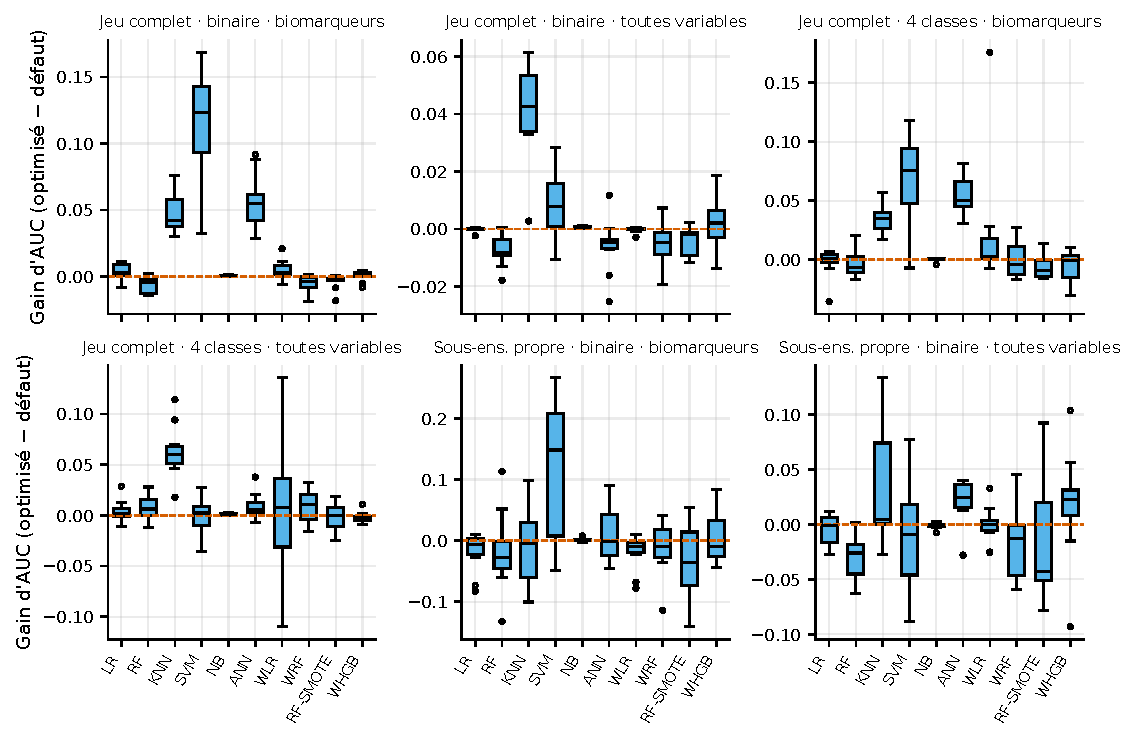
\includegraphics[width=0.78\textwidth]{../figures/nested_gain.pdf}
\caption{Gain d'AUC (optimisé $-$ défaut) sur les 10 plis externes de la validation croisée imbriquée, par modèle et par cadre.}\label{fig:nested}\end{figure*}

\textbf{Comparaison des modèles.} Dans le régime complet, le test de Friedman rejette l'égalité des six classifieurs de base ($\chi^2\approx 46$--$49$, $p<10^{-3}$) et la RF est significativement supérieure à chacun des autres (Conover--Holm, $p<10^{-3}$ ; seule exception, RF--KNN optimisé sur les biomarqueurs seuls : $p=0{,}047$), ce qui \textbf{reproduit} le résultat de l'article (tableau~\ref{tab:friedman}). Dans le régime propre, le test n'est significatif que par défaut ($p_F=0{,}015$, seule la paire RF--KNN ressort) et plus du tout après optimisation ($p_F=0{,}63$) : les six classifieurs y sont indiscernables.

\begin{table*}[t]\centering\caption{Tests de Friedman et post-hoc de Conover (valeurs $p$ corrigées de Holm) sur les 10 plis externes : à gauche les six classifieurs de base (RF contre chaque autre modèle), à droite les modèles pondérés (WRF contre WLR et RF-SMOTE).}\label{tab:friedman}
\scriptsize\setlength{\tabcolsep}{2.4pt}\begin{tabular}{llccccccccccc}
\toprule
& & \multicolumn{7}{c}{Six classifieurs de base (RF contre\,\dots)} & \multicolumn{4}{c}{Modèles pondérés (WRF contre\,\dots)} \\\cmidrule(lr){3-9}\cmidrule(lr){10-13}
Cadre & Variante & $\chi^2$ & $p_F$ & LR & KNN & SVM & NB & ANN & $\chi^2$ & $p_F$ & WLR & RF-SMOTE \\
\midrule
Complet, binaire, toutes var. & défaut & 48,8 & $<\!10^{-3}$ & $<\!10^{-3}$ & $<\!10^{-3}$ & $<\!10^{-3}$ & $<\!10^{-3}$ & $<\!10^{-3}$ & 15,8 & $<\!10^{-3}$ & $<\!10^{-3}$ & 0,081 \\
 & optimisé & 47,3 & $<\!10^{-3}$ & $<\!10^{-3}$ & $<\!10^{-3}$ & $<\!10^{-3}$ & $<\!10^{-3}$ & $<\!10^{-3}$ & 15,0 & $<\!10^{-3}$ & $<\!10^{-3}$ & 1,000 \\
\midrule
Complet, 4 classes, toutes var. & défaut & 48,0 & $<\!10^{-3}$ & $<\!10^{-3}$ & $<\!10^{-3}$ & $<\!10^{-3}$ & $<\!10^{-3}$ & $<\!10^{-3}$ & 15,8 & $<\!10^{-3}$ & $<\!10^{-3}$ & 0,081 \\
 & optimisé & 47,4 & $<\!10^{-3}$ & $<\!10^{-3}$ & $<\!10^{-3}$ & $<\!10^{-3}$ & $<\!10^{-3}$ & $<\!10^{-3}$ & 15,8 & $<\!10^{-3}$ & $<\!10^{-3}$ & 0,081 \\
\midrule
Complet, binaire, biomarq. & défaut & 48,6 & $<\!10^{-3}$ & $<\!10^{-3}$ & $<\!10^{-3}$ & $<\!10^{-3}$ & $<\!10^{-3}$ & $<\!10^{-3}$ & 15,0 & $<\!10^{-3}$ & $<\!10^{-3}$ & 1,000 \\
 & optimisé & 46,3 & $<\!10^{-3}$ & $<\!10^{-3}$ & 0,047 & $<\!10^{-3}$ & $<\!10^{-3}$ & $<\!10^{-3}$ & 15,2 & $<\!10^{-3}$ & $<\!10^{-3}$ & 0,398 \\
\midrule
Propre, binaire, toutes var. & défaut & 14,1 & 0,015 & 1,000 & 0,024 & 1,000 & 1,000 & 0,059 & 4,2 & 0,122 & 0,137 & 0,339 \\
 & optimisé & 3,4 & 0,631 & 1,000 & 1,000 & 1,000 & 1,000 & 1,000 & 2,6 & 0,273 & 0,541 & 0,655 \\
\bottomrule
\end{tabular}
\end{table*}

Parmi les modèles pondérés (partie droite du tableau~\ref{tab:friedman}), la WRF est significativement meilleure que la WLR dans le régime complet ($p<10^{-3}$), mais pas que RF-SMOTE au seuil de 5\,\% ($p=0{,}081$ à quatre classes, par défaut comme optimisée) : la supériorité de la WRF sur RF-SMOTE n'apparaît qu'au seuil de 10\,\%, comme dans l'article (qui retient $\alpha=0{,}1$ pour toutes les variables).

\textbf{Jeux de variables.} Pour la WRF optimisée, ajouter les variables cliniques n'améliore pas l'AUC en binaire dans le régime complet ($+0{,}002$, $p_W=0{,}70$) : les seuls biomarqueurs suffisent, ce qui contredit l'article. L'ajout aide à quatre classes ($+0{,}025$, $p_W=0{,}020$, $p_{NB}=0{,}13$) et nettement dans le régime propre ($+0{,}090$, $p_W=0{,}004$, $p_{NB}=0{,}038$) : sans doublons, l'essentiel du signal vient des variables cliniques.

\subsection{Discussion}
\paragraph{Qui gagne à l'optimisation ?} Les modèles dont les réglages par défaut sont mal adaptés (KNN, SVM, ANN) gagnent de $+0{,}04$ à $+0{,}12$ d'AUC dans le régime complet ; les ensembles d'arbres, déjà proches de leur plafond, ne gagnent rien (RF et WRF : $-0{,}007$ à $+0{,}009$, non significatif ou négatif) et leur AUC varie peu autour des bons réglages (figure~\ref{fig:hp}). Grille, recherche aléatoire et TPE donnent des scores équivalents à budget comparable (tableau~\ref{tab:time}) : la valeur ajoutée dépend du \emph{modèle} plus que de la \emph{stratégie} de recherche. Dans le régime propre, les écarts entre configurations (0,66--0,72) sont du même ordre que l'écart-type entre plis (0,06--0,08) : la sélection suit surtout le bruit, d'où le gain négatif de la RF.

\paragraph{Une optimisation qui apprend la fuite ?} Dans le régime complet, les gains vont aux modèles capables d'\emph{interpoler} des valeurs dupliquées, et les réglages choisis sont de capacité maximale (arbres entièrement développés, KNN pondéré par la distance, SVM à $C\approx 46$). Cinq indices concordent avec l'hypothèse de fuite : (i) la RF atteint 0,94 avec trois biomarqueurs presque non corrélés à la cible ($|r|\leq 0{,}06$), alors que LR et NB restent à 0,5 ; (ii) les biomarqueurs seuls égalent les toutes variables ; (iii) l'optimum de profondeur est « le plus profond » dans le régime complet, mais s'inverse dans le régime propre (figure~\ref{fig:hp}) ; (iv) l'importance par permutation (figure~\ref{fig:perm}) place P66, MOTS-c et Humanin en tête dans le régime complet, puis s'annule pour eux dans le régime propre où le diabète domine ; (v) l'AUC tombe de 0,94 à 0,60 (biomarqueurs seuls) sans lignes à valeurs partagées. La conclusion de l'article selon laquelle les biomarqueurs sont les variables les plus importantes n'est donc \emph{pas robuste} sur ce fichier. Nous ne savons pas si les données de l'article ont le même défaut ; sa méthode d'imputation par classes en fait toutefois un point à vérifier.

\begin{figure*}[t]\centering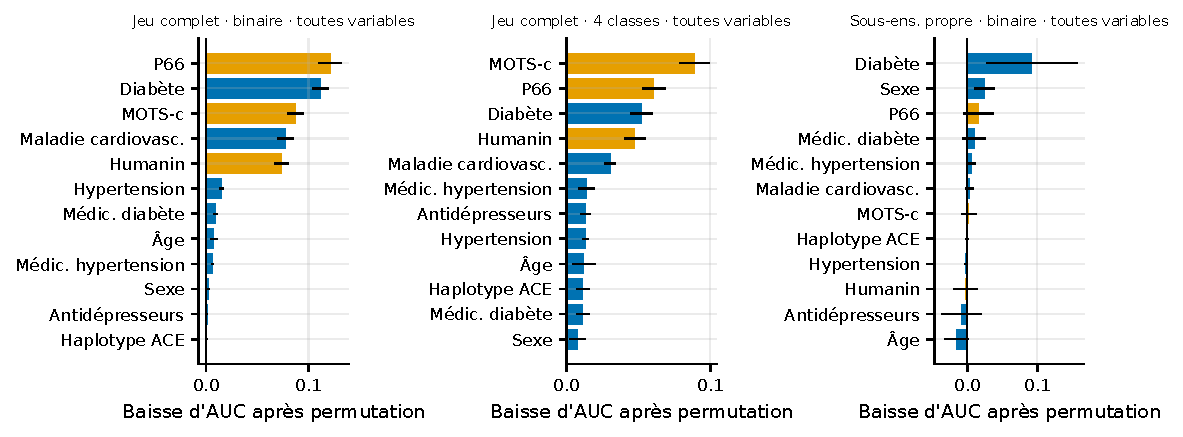
\includegraphics[width=0.92\textwidth]{../figures/permutation_importance.pdf}
\caption{Importance par permutation pour la WRF optimisée (30 permutations, jeu de test) ; orange : biomarqueurs.}\label{fig:perm}\end{figure*}

\paragraph{Limites et cas d'échec.} Le régime propre ne compte que 228 lignes (62 déprimées) : la puissance statistique est faible, la tâche à quatre classes y est impossible (3 cas sévères) et le choix du sous-ensemble peut introduire un biais de sélection. La WLR s'effondre à quatre classes (poids jusqu'à 21, exactitude 0,48) ; NB et LR sont inopérants sur les biomarqueurs seuls ; le SVM par défaut est sous le hasard sur les biomarqueurs du régime propre (0,44) et l'optimisation le ramène au hasard (0,55, non significatif). L'apport de la pondération reste modeste, y compris pour les métriques sensibles au déséquilibre (exactitude équilibrée de la WRF : 0,644 à 0,667 contre 0,648 pour la RF).
